%! TEX root = ./masm12_report.tex
\documentclass[a4paper, 12pt]{article}
\input{~/preamble.latex}
\usepackage[authoryear,round]{natbib}
\usepackage{subcaption}

\title{A Latent Poisson Model of Timing Prediction Markets}
\author{Erik Göransson-Gaspar}
\date{MASM12 Non-Linear Time Series Analysis \\
January 2026}

\begin{document}
\maketitle
\tableofcontents

\section{An Overview of Prediction Markets}
Actors in prediction markets trade contracts whose payout is tied to the outcome of underlying real-world events. The standard type of contract pays out one U.S. dollar to the holder if the underlying event occurs and nothing otherwise. These markets were introduced in their modern form by researchers at the University of Iowa to predict the 1988 U.S. presidential election. Since then they have attracted significant attention from economists. \citet{WolfersZitzewitz2006} show that under standard conditions the equilibrium market price is a budget-weighted average of traders' beliefs about the underlying event. This justifies the interpretation of market prices as estimates of the probability that the event will occur. They also note that prediction markets are quick to incorporate new information and often outperform traditional forecasts based on polls or expert opinions. It is well-established that prediction market prices exhibit the same behaviors characteristic of other financial time series, e.g. uncorrelated returns and clustered volatility. \citep{majumder2009} \citet{horn2014} provides a thorough overview of the literature.

Prediction markets are currently enjoying a period of significant interest, starting around the 2024 U.S. Presidential election. With a trading volume of over one billion dollars, the market for this election on the platform Polymarket became the most active in history. This platform, together with its competitor Kalshi, are the current leading prediction market providers. Kalshi is registered with U.S. regulators and relies on a centralized order book, while Polymarket uses a decentralized blockchain-based architecture with an automatic market maker to ensure price consistency between related contracts. The economic literature on prediction markets has historically been interested in how to best construct markets useful for, e.g., informing policy makers. With the recent appearance of large prediction market providers, I argue that it now makes sense to consider prediction markets not as design problems, but as financial instruments in their own right to be modeled with tools developed for derivative pricing. There has been previous work in this direction. \citet{archakIpeirotis2009} suggest pricing prediction market prices as derivatives on latent \textit{ability processes}, modeled as Itô diffusions. This allows for closed form expressions of price volatility while preserving the martingale property of the price process. Another promising approach is pursued by \citet{dalen2025}, who proposes modeling the log-odds of the market price as a jump-diffusion process. In the present report I propose a model in this spirit for an exotic type of prediction market. 

Although the current market providers primarily make a profit from retail traders using their platforms for mere gambling, prediction markets are worth studying due to three use cases in particular. First, they provide analysts with robust probability estimates for a large range of events, which can inform more qualified decision making. Prediction markets also offer a novel opportunity to hedge specific exposures, especially policy-related risks. Good models of market prices are needed to do this effectively. Finally, these markets should be of particular interest to statisticians, as they provide easily accessible input signals to more complex models. An unemployment model, for example, could account for uncertainty about future central bank policy by including relevant prediction market prices as exogenous variables.

The standard prediction market contract is based on a question of type "Will event X occur on time T?", e.g. "Will Trump win the U.S. presidential election on election day?". The price history for this market is shown in Figure \ref{fig:trump2024price}. Since the winner of the election is not certain until election day, the market price remains far away from zero or one, until the market resolves with a discrete jump. In the following I distinguish between the \textit{yes-price} of a market, which is the price of a contract which pays out if the underlying event occurs and the market resolves to \textit{yes}, and the \textit{no-price}, which is the price of a contract with the opposite pay-out structure. Both yes- and no-contracts are typically tradable. With the new prediction market platforms, another type of market have recently been introduced, based on questions of the type "Will event X occur before event T?". The outcome of some event is not in question here, but rather the timing. I call such markets \textit{timing markets} to distinguish them from the standard \textit{outcome markets}. Figure \ref{fig:khomeini2025price} shows the price history for the timing market "Khamenei out as Supreme Leader of Iran in 2025?". The large price increase in June corresponds to the U.S.-Israeli attacks on Iran. Timing markets exhibit an entirely different behavior than outcome markets. If the underlying event does not occur, then \textit{ceteris paribus} the price tends slowly to zero as the end date \(T\) approaches. If the event occurs, this will instead manifest as a discrete jump to a price of one. Because of this convergence behavior, timing markets should not be modeled in the same way as outcome markets. I here present a novel model for timing markets, based on a latent Poisson process. As far as I know, these markets have not yet been studied in the literature. In the next section I will elaborate on this model and suggest both simulation and estimation procedures. Section 3 contains an analysis of the market "Khamenei out as Supreme Leader of Iran in 2025?", which I use to illustrate the use-cases for such a model. The final section concludes with a discussion of model limitations and promising avenues for future work. 

\begin{figure}[tbp]
  \centering

  \begin{subfigure}{\textwidth}
    \centering
    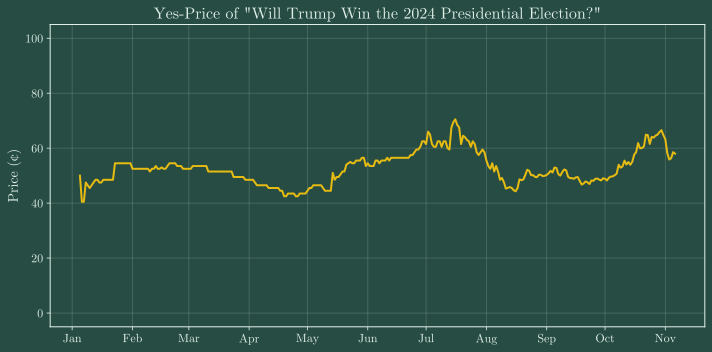
\includegraphics[width=\textwidth]{trump2024daily.pdf}
    \caption{Yes-price of the outcome market "Will Trump Win the 2024 Presidential Election?".}
    \label{fig:trump2024price}
  \end{subfigure}
  \par\vspace{1cm}
  \begin{subfigure}{\textwidth}
    \centering
    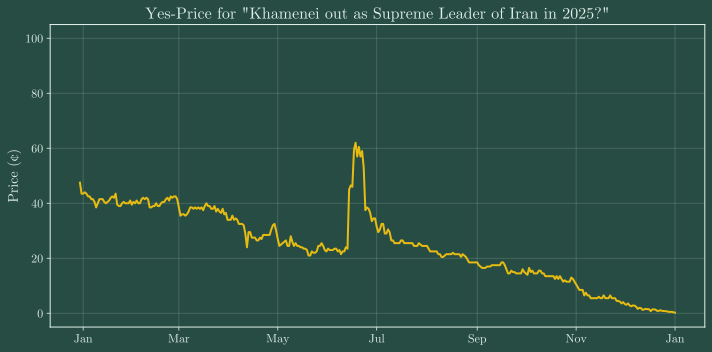
\includegraphics[width=\textwidth]{khameiniOut2025.pdf}
    \caption{Yes-price of the timing market "Khamenei out as Supreme Leader of Iran in 2025?".}
    \label{fig:khomeini2025price}
  \end{subfigure}

  \caption{Examples of high liquidity outcome (a) and timing (b) prediction markets. Note the different convergence behaviors.}
  \label{fig:main}
\end{figure}

\section{Pricing Timing Contracts}
\subsection{A Latent Poisson Model}
Researchers studying defaultable corporate bonds have developed methods to price contracts whose pay-out depends on the occurrence of an event. One family of these models, so called \textit{structural}, suppose that corporate default arrives by a Poisson process. \citep{bakshi2022} I suggest using a model of this type to price timing prediction markets. 

Consider a timing prediction market with end date \(T\) and suppose that the underlying event (and with it market resolution) arrives by a Poisson process with intensity process~\(\lambda_t\). Let \(R\) denote the resolution time of the market. The no-price at time \(t\) consistent with interpreting prices as probabilities is then 
\begin{equation*}
  \pi_t^\text{no} = \mathbb{P}\left[ R> T | \mathcal{F}_t \right] = \mathbb{E}\left[e^{-\int_t^T\lambda_s \mathrm{d}s} | \mathcal{F}_t \right],
\end{equation*}
where \(\pi_t^\text{no}\) is adapted to the filtration \(\mathcal{F}_t\). In this report I will not account for discounting of future pay-outs when calculating prices. Since most prediction markets do not last longer than a year, any discounting effect would be small. 

By imposing dynamics on the intensity process \(\lambda_t\) we can derive properties of the price process. I will suppose that \(\lambda_t\) follows a mean-reverting Ornstein-Uhlenbeck process with dynamics
\begin{equation*}
  \mathrm{d}\lambda_t = -\kappa(\lambda_t - \mu)\mathrm{d}t + \sigma \mathrm{d}W_t, \quad \kappa,\sigma>0
\end{equation*}
where \(W_t\) is a standard Wiener process. Note that the Ornstein-Uhlenbeck process is not prevented from becoming negative, which would result in invalid intensity values. We avoid this by clipping the process to never be less than zero when simulating the model. As a consequence, all results derived below are approximations of the model actually implemented, but with realistic parameter values I do not expect this to introduce an unacceptable error. This clipping could be avoided by instead letting the intensity \(\lambda_t\) be a Cox-Ingersoll-Ross process. It is, however, much harder to study analytically than the Ornstein-Uhlenbeck process. I leave this for future work. 

The Gaussian transition density of the Ornstein-Uhlenbeck process allows us to derive the dynamics of the price process. Solving the SDE governing the intensity process yields
\begin{equation*}
  \lambda _s \vert \mathcal{F}_t \sim \mathcal{N}\left(\mu + e^{-\kappa (s-t)}(\lambda_t-\mu ), \frac{\sigma^2}{2\kappa }\left[1-e^{-2\kappa (s-t)} \right]\right), \quad t<s\leq T.
\end{equation*}
It follows that the distribution of the forward integral \(\int_t^T \lambda_s \mathrm{d}s\) conditional on \(\mathcal{F}_t\) is also Gaussian and \(\pi_t^\text{no}\) is the expected value of a log-normal random variable. By applying Itô's lemma we get 
\begin{equation*}
  \,\mathrm{d}\pi^\text{no}_t = \pi^\text{no}_t\left[ \mu +L_1(\log\pi^\text{no}_t + L_2) \right]\,\mathrm{d}t + \pi^\text{no}_t \frac{\sigma (1 - e^{-\kappa \tau })}{\kappa }\,\mathrm{d}W_t,
\end{equation*}
where \(\tau := T-t\) and 
\begin{equation*} 
  L_1 := \frac{\kappa }{e^{-\kappa \tau }-1}, \quad L_2:=\mu \tau -\frac{V}{2},
\end{equation*}
\begin{equation*}
V := \frac{\sigma ^2}{2\kappa ^3}\left( 2\kappa \tau +4e^{-\kappa \tau }-e^{-2\kappa \tau } - 3 \right).
\end{equation*}
A key benefit of this model is that we also get an invertible relationship between the no-price \(\pi_t^\text{no}\) and intensity \(\lambda_t\):
\begin{equation*}
  \lambda_t = \mu + L_1(\log\pi_t^\text{no} + L_2). 
\end{equation*}
Note that the drift term of the price dynamics is exactly \(\pi_t^\text{no}\lambda_t > 0\); timing market prices are not martingales, conditional on non-resolution, but instead drift towards a no-price of one. This is exactly what we observed in real timing markets. We also see that the relative volatility 
\begin{equation*}
  \frac{\mathrm{d}\pi_t^\text{no}}{\pi_t^\text{no}} = \frac{\sigma(1-e^{-\kappa \tau})}{\kappa}
\end{equation*}
is decreasing as \(t \rightarrow T\). We have derived the price dynamics implied by the latent Poisson model and found that it reproduces the observed convergence behavior of timing prediction markets. In the rest of this section I will present procedures for simulating this model and for fitting its parameters to real price series.

\subsection{Simulation}
We can easily simulate from the above model by discretizing the price dynamics with an Euler-Maruyama scheme on a time grid \(t=t_1, t_2, \dots, t_n = T\). This yields
\begin{equation*}
  \pi^\text{no}_{k+1} = \pi_k^\text{no} + \pi_k^\text{no}\Delta\left[\mu + L_1(\log\pi^\text{no}_k + L_2)\right] + \pi^\text{no}_k \frac{\sigma}{\kappa}(e^{-\kappa\tau}-1)Z
\end{equation*}
where \(\Delta\) is the size of the time step and \(Z \sim \mathcal{N}(0, \Delta)\). We write \(\pi_k^\text{no} := \pi_{t_k}^\text{no} \). These dynamics are conditional on the market not resolving. Therefore, when simulating sample \(k+1\) we first determine whether the market resolved in the time interval \([t_k, t_{k+1}]\), which approximately occurs with probability
\begin{equation*}
  1 - e^{-\lambda_k\Delta } = 1 - \pi_k^{-\Delta L_1}e^{-\Delta (\mu +L_1L_2)}.
\end{equation*}
This uses the approximation \(\int_{t_k}^{t_{k+1}}\lambda_s\mathrm{d}s \approx \lambda_k\Delta\), with the same shorthand \(\lambda_k := \lambda_{t_k}\) as for the price process. When simulating we wish to avoid prices implying a negative intensity \(\lambda_t\). This occurs when
\begin{equation*}
0 > \lambda_t = \mu + L_1(\log\pi_t + L_2) \iff \pi_t > e^{-(\mu / L_1 + L_2)}.
\end{equation*}
There are multiple ways to handle such samples. I have chosen to simply discard them and draw new ones until one is valid. This is equivalent to sampling conditional on \(\lambda_t \geq 0\). Taken together, this results in a simulation procedure which respects the resolution and convergence behavior of the model.

\subsection{Parameter Estimation}
We have above derived a SDE governing the price dynamics. I believe it to be solvable exactly, at least up to numerical integration, but I have for the present report chosen to pursue a simpler approximation. The Euler-Maruyama scheme derived in the previous section gives us an approximate transition probability density for the price process. We have that
\begin{equation*}
\pi^{\text{no}}_{k+1}\mid \pi^{\text{no}}_k \sim 
\mathcal{N}\!\left(
\pi^{\text{no}}_k
+ \pi^{\text{no}}_k \Delta
\left[\mu + L_1\!\left(\log \pi^{\text{no}}_k + L_2\right)\right],
\;
\frac{(\pi^{\text{no}}_k)^2 \sigma^2 \Delta}{\kappa^2}
\left(e^{-\kappa \tau}-1\right)^2
\right).
\end{equation*}
This allows us to use the quasi-maximum likelihood estimator of the parameters. These estimates ought to be acceptable if the discretization does not introduce significant error. The mean-reversion strength \(\kappa\) enters the likelihood non-linearly through terms of the form \(e^{-C\kappa\tau}\). Because of this, I expect it to be difficult to identify, which makes the numerical quasi-likelihood maximization especially sensitive to initial values. In order to find good initial values we first perform a partial optimization, letting \(\mu\) and \(\sigma\) be free, while fixing \(\kappa\). We do this for a grid of reasonable values of \(\kappa \in (0, 5)\). The set of parameters resulting in the highest quasi-likelihood was then used as initial values for a full optimization of all three parameters simultaneously. To enforce positivity on \(\sigma\) and \(\kappa\), we optimize their logarithm.

To evaluate the performance of this estimation procedure, I simulated 1 000 timing markets from the model presented above with the parameters \(\mu~=~1,~\sigma~=~\kappa~=~1/2\) and an initial yes-price of 50¢. Each market was simulated for 1 000 steps or until resolution, whichever came first; to ensure sufficient data I forced each simulated market to contain at least 500 samples. I also removed 17 outlier runs, which had at least one parameter estimate with an absolute value greater than 50. The mean and standard deviation of the remaining 983 estimates are shown in Table \ref{tbl:sim_estimates}. We see that both the mean $\mu$ and volatility $\sigma$ are fairly well-estimated, although with a significant spread between runs. As expected, the mean-reversion strength $\kappa$ is estimated poorly and with massive variation. In the future, I would like to investigate how robust the model is to changes in $\kappa$; perhaps an \textit{a priori} fixed value would improve real-world performance.

\begin{table}[hbt]
\centering
\caption{Summary of 983 Parameter Estimations (17 out of 1000 runs removed as outliers)}
\label{tbl:sim_estimates}
\begin{tabular}{cccc}
\toprule
Parameter & True Value & Estimate & St.d. \\
\midrule
$\mu$     & 1.00 & 1.06 & 2.37 \\
$\sigma$ & 0.50 & 1.62 & 1.20 \\
$\kappa$ & 0.50 & 5.55 & 5.40 \\
\bottomrule
\end{tabular}
\end{table}

\section{Analysis of Real Market Prices}
With both simulation and estimation procedures in place, we are ready to explore applications of the latent Poisson model. To demonstrate these, we will fit the model to the market shown in Figure \ref{fig:khomeini2025price} based on the question "Khamenei out as Supreme Leader of Iran in 2025?" The procedure described in Section 2.3 yields the following parameter estimates, with Wald 95 \%-confidence intervals:
\begin{equation*}
  \hat{\mu} = 0.69\,\, [0.57, 0.80], \quad 
  \hat{\sigma} = 2.85\,\, [2.59, 3.15], \quad
  \hat{\kappa} = 3.61\,\, [2.34, 5.56].
\end{equation*}
The Wald confidence intervals are based on a Gaussian approximation of the parameter distribution. This is appropriate only if these distributions are symmetric, which is not necessarily the case for a highly non-linear model such as this one. One could diagnose these by looking at the profile likelihoods of the parameters, and if more accurate error estimates are needed, then one could use these to compute profile likelihood-based confidence intervals instead. Equipped with parameter estimates, we can utilize the fitted model in various ways.
\newpage
\subsection{Reconstructing Intensity and Volatility}
\begin{figure}
  \centering
  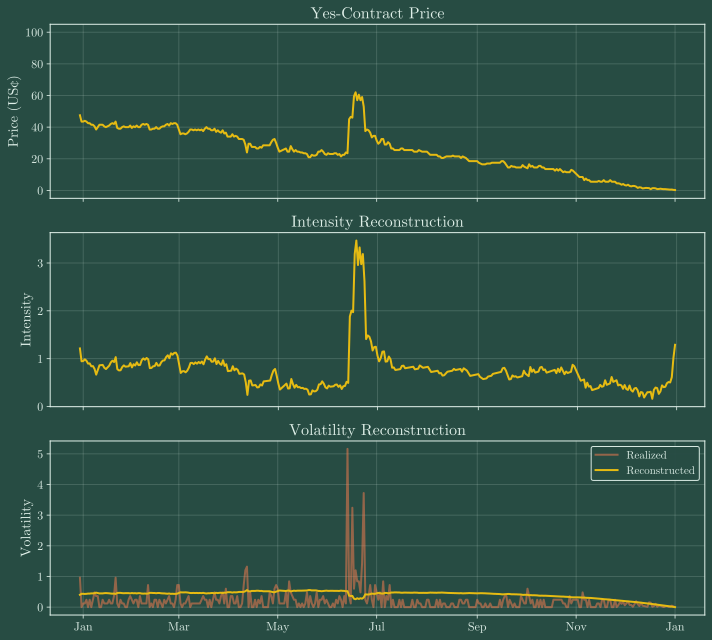
\includegraphics[width=\textwidth]{reconstruction.pdf}
  \vspace{-3em}
  \caption{Intensity and volatility series reconstructed from historic prices for the market "Khamenei out as Supreme Leader of Iran in 2025?".}
  \label{fig:reconstructions}
\end{figure}

One of the key benefits of assuming that the intensity \(\lambda_t\) follows an Ornstein-Uhlenbeck process is that we get closed expressions for both the intensity and the volatility \(v_t\) in terms of the no-price \(\pi_t^\text{no}\). We have
\begin{equation*}
   \lambda_t = \mu + L_1(\log\pi_t^\text{no} + L_2)\quad\text{and}\quad v_t = \frac{\pi_t^\text{no} \sigma}{\kappa}(1-e^{-\kappa\tau}).
\end{equation*}
This allows us to reconstruct intensity and volatility series from historic prices. Such reconstructions for the market "Khamenei out as Supreme Leader of Iran in 2025?" are shown in Figure \ref{fig:reconstructions}. As expected, we see a spike in intensity coinciding with the increased yes-price in June. The corresponding change in the volatility is negative, because it is proportional to the no-price. The reconstructed volatility is plotted alongside the unsmoothed realized volatility, which is a very noisy estimator. The fact that the reconstruction is consistently higher than the realized volatility, except for during the spike when it is considerably lower is a first indication that the latent Poisson model does not capture the full volatility dynamics of the market prices. This is however hard to judge without any confidence intervals. Uncertainty in the reconstructions derives from the distribution of the parameter estimates. By the samma normal approximation underlying the Wald confidence interval, we could use the delta-method to derive approximate confidence intervals also for the reconstructions. I leave this for future work.

\subsection{Monte Carlo Forecasts}
The fitted model does not only allow us to reconstruct historic intensity and volatility, but also to forecast future values. The simplest way to do this is to simulate the process a large number of time from some starting price, using the procedure described in Section 2.2. These Monte Carlo samples then approximate the model-implied distribution of future prices. Such forecasts, conditional on the market not resolving, are shown in Figure \ref{fig:forecasts}, from 6 September and 37 days forward together with 95 \% confidence intervals. I ran 1 000 Monte Carlo simulations. To avoid data leakage, the model parameters were re-estimated with data only available up until that time. The new parameters (with 95 \% Wald confidence intervals)
\begin{equation*}
\hat{\mu} = 0.83\;[0.75,\,0.92], \quad
\hat{\sigma} = 20.60\;[19.72,\,21.53], \quad
\hat{\kappa} = 27.81\;[25.93,\,29.83]
\end{equation*}
were significantly different from the ones estimated on the full data. This is another indication that the estimation procedure described in Section 2.3 is inadequate. Reconstructed intensities and volatilities using both sets of parameters are included in the figure.


\begin{figure}
  \centering
  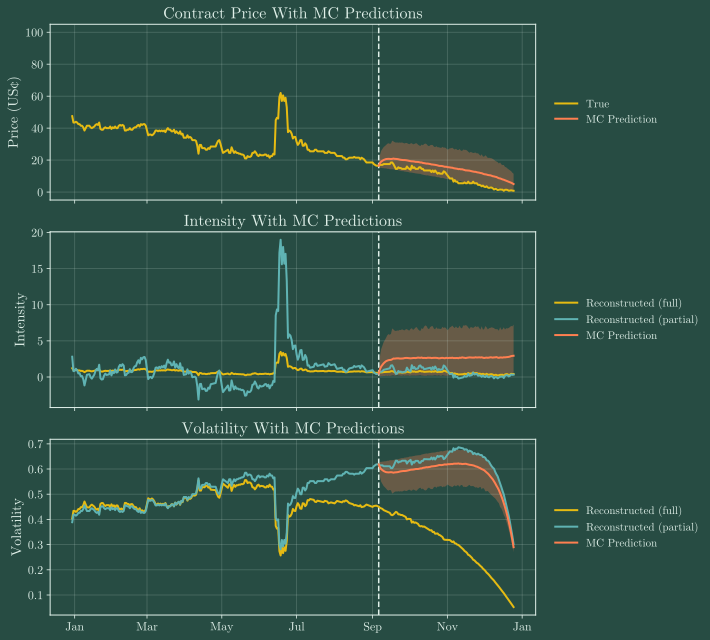
\includegraphics[width=\textwidth]{forecasts.pdf}
  \caption{Monte Carlo forecasts of market price, intensity and volatility ($n=1000$) using only data available at the forecasting time 6 September. Confidence intervals are derived from the empirical quantiles of the Monte Carlo samples. Reconstructed intensity and volatility series, derived from parameters estimated on both the full and partial data, are included.}
  \label{fig:forecasts}
\end{figure}

The price forecasts are remarkably accurate. Note that although the level of the volatility forecast is very different from the reconstruction, due to the large difference in parameter estimates from the full and partial data, the dynamics seem to be well-captured. The Monte Carlo simulations used to produce these forecasts are conditioned on the market not resolving within the forecast horizon; the same methodology can also be used to get fine-grained estimates of when the market will resolve.

\subsection{Fine-Grained Prediction of Resolution Probability}
Consider a timing market with end date \(T\) and denote its resolution time by \(R \leq T\). At some time \(t_0 < R\), the probability that the market will resolve before some later time \(t_1>t_0\) is
\begin{equation*}
  \mathbb{P}[R \leq t_1 | \mathcal{F}_{t_0}] = 1-\mathbb{E}\left[e^{-\int_{t_0}^{t_1}\lambda_s\mathrm{d}s}\vert\mathcal{F}_{t_0}\right].
\end{equation*}
I believe that it is possible to express this in terms of the model parameters and the no-price \(\pi_{t_0}^\text{no}\), but I have not pursued this further. Under the assumed model, we can instead estimate this probability by simulating a large number of markets, starting at \(\pi_{t_0}^\text{no}\), and simply counting the proportion of markets which resolve before time \(t_1\). Figure \ref{fig:prob_sim} contains these estimates for a range of horizons \(t_1-t_0\) on simulated data. Note that the probability of the market resolving before \(t_1\) converges to the yes-price \(\pi_{t_0}^\text{yes}\) at time \(t_0\) as \(t_1 \rightarrow T\). This corresponds to the probability estimates approaching the grey horizontal line. Figure \ref{fig:prob_real} shows these estimates from the market "Khamenei out as Supreme Leader of Iran in 2025?", using parameters estimated from data available at time \(t_0 = \) 6 September. These estimates do not converge to the market price \(\pi_{t_0}^\text{yes}\); many more simulations resolve than is expected given the market price. This indicates a serious misscalibration of the model. In order to pin down this issue, we will next consider a number of ways to evaluate model performance.

\begin{figure}[tbp]
  \centering

  \begin{subfigure}{0.48\textwidth}
    \centering
    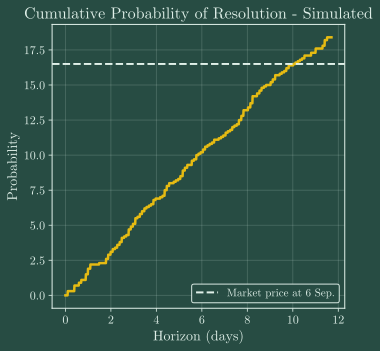
\includegraphics[width=\textwidth]{prob_sim.pdf}
    \caption{Simulated data}
    \label{fig:prob_sim}
    \vspace{1em}
  \end{subfigure}
  \hfill
  \begin{subfigure}{0.48\textwidth}
    \centering
    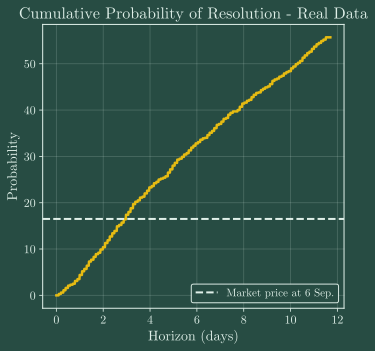
\includegraphics[width=\textwidth]{prob_real.pdf}
    \caption{Real data from the market "Khamenei out as Supreme Leader of Iran in 2025?".}
    \label{fig:prob_real}
  \end{subfigure}

  \caption{Estimated probability of resolving within a horizon from time \(t_0 =\) 6 September for (a) well-calibrated simulated data and (b) real data from the market "Khamenei out as Supreme Leader of Iran in 2025?".}
\end{figure}

\subsection{Goodness-of-Fit}
The approximate transition density derived in Section 2.3 gives us a one-step prediction distribution, conditional on the market not resolving. Consider the residuals \(r_{k+1} := \pi_{k+1}^\text{no} - \pi_k^\text{no}\). The model implies that they have a conditional distribution
\begin{equation*}
  r_{k+1}|\pi_k^\text{no} \sim 
\mathcal{N}\!\left(
\pi^{\text{no}}_k \Delta
\left[\mu + L_1\!\left(\log \pi^{\text{no}}_k + L_2\right)\right],
\;
\frac{(\pi^{\text{no}}_k)^2 \sigma^2 \Delta}{\kappa^2}
\left(e^{-\kappa \tau}-1\right)^2
\right).
\end{equation*}
If the latent Poisson model fits the data well, then the standardized residuals ought to be uncorrelated and standard Gaussian-distributed. Figure \ref{fig:diagnostics} shows a histogram and quantile-quantile plot of the residuals. Their mean is -0.05 and their standard deviation is 1.17, which indicates good model fit. The distribution is symmetric with heavy tails, which is typical of financial time series. The figure also contains autocorrelation functions of the residuals and their squares. Although it is not definitive, they indicate that some correlation remains which the model has not accounted for. Note that this is in-sample validation, since the parameter estimates used to make one-step predictions are fitted to the entire price series. A more systematic evaluation of this model would have to include out-of-sample validation on multiple markets. 

\begin{figure}[t]
  \centering
  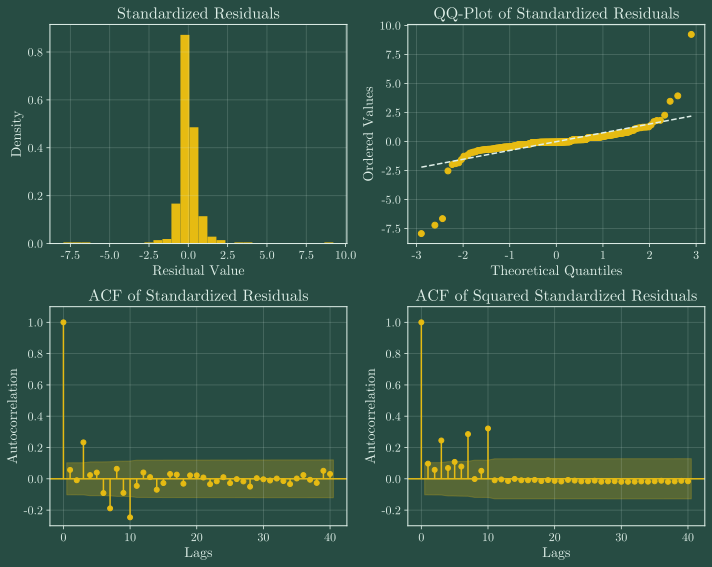
\includegraphics[width=\textwidth]{diagnostics.pdf}
  \caption{Histogram, quantile-quantile plot, and autocorrelation function of standardized residuals and their squares. The one-step prediction residuals were computed from the market "Khamenei out as Supreme Leader of Iran in 2025?".}
  \label{fig:diagnostics}
\end{figure}

We can get a closer look at how well the model predicts price volatility by considering the coverage of prediction intervals. The Gaussian one-step prediction distribution allows us to easily construct approximate prediction intervals for various confidence levels. If the model is well-calibrated, then an \(\alpha\)-level prediction interval should contain the true value a fraction \(\alpha\) of the times. We can compute this coverage fraction across the entire price history for a range of confidence levels. This is done for the market "Khamenei out as Supreme Leader of Iran in 2025?" in Figure \ref{fig:ci_coverage}. Ideal model calibration would manifest as a diagonal line in such a plot. Instead, we see that the latent Poisson model systematically implies prediction intervals that are too wide, corresponding to an overestimation of the volatility. This agrees with what we observed when comparing the reconstructed volatility with the realized volatility in Figure \ref{fig:reconstructions}. I believe that this is caused by the large price spike in June 2025. The true price volatility increased, as is seen in the realized volatility, which the stationary latent Poisson model could not accommodate. Instead, this caused the quasi-maximum likelihood estimator to inflate the baseline volatility of the entire price series, leading to the overestimation we observe. If this interpretation is correct, then the model could be improved by incorporating a non-stationary component. This could, for example, be a jump-term in the intensity-dynamics or time-varying parameters.

\begin{figure}[t]
  \centering
  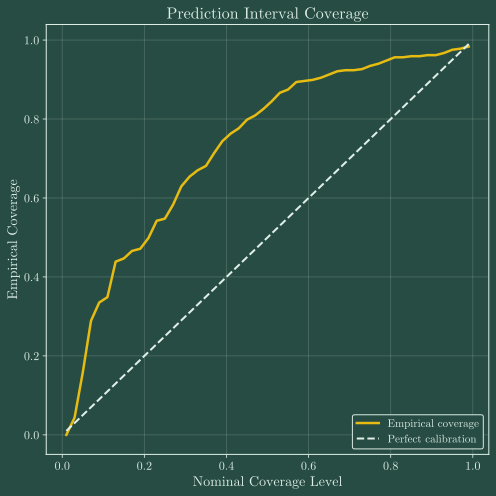
\includegraphics[width=0.6\textwidth]{ci_coverage.pdf}
  \caption{Empirical coverage of Gaussian one-step prediction intervals for the market “Khamenei out as Supreme Leader of Iran in 2025?” plotted against nominal coverage, with the diagonal indicating perfect calibration.}
  \label{fig:ci_coverage}
  
\end{figure}

\section{An Insufficient but Promising Framework}
In this report I have presented a novel model of timing prediction markets, which are previously unstudied in the literature. By letting market resolution be driven by a latent Poisson process with stochastic intensity, the model reproduces the convergence behavior of real timing markets. Although I have presented a general framework, it is simple to adapt it to the prediction of specific markets, e.g. by incorporating external inputs driving the intensity process.

While the latent Poisson model captures the qualitative behavior of timing markets, it is too simple to make good forecasts. It consistently overestimates the price volatility of the market we have studied and simulations resolve significantly more often than the real market price implies. I believe that the key flaw of the model is its stationarity. By adding a time-varying component, the model would be better able to adapt to the dynamics of real market prices. This could be done by letting parameters vary with time using a particle filter, by adding a jump-component to the price dynamics, or by including a Heston-style stochastic volatility. There are also more minor improvements to be made to the model. The Ornstein-Uhlenbeck intensity process should be replaced with a Cox-Ingersoll-Ross process to avoid errors due to conditioning on the intensity being non-negative. The estimation procedure, which is currently quite unstable, also needs improvement. This could be achieved by performing exact maximum likelihood estimation and by finding a more robust way to deal with the hard-to-identify mean-reversion parameter \(\kappa\). There is also work to be done in deriving proper uncertainty measures for all model-implied estimates. These improvements are all important to ensure the models usefulness in applications.

The existence of a model for timing prediction markets facilitates their utilization in three key ways. It provides novel information to analysts, by allowing them to make forecasts and providing them with fine-grained estimates of when the underlying event is most likely to occur. The model also enables the use of timing markets for reducing exposure to the underlying event, by providing volatility forecasts needed for optimal hedging. Finally, the latent Poisson model enables the inclusion of timing market prices as inputs to other statistical models, because it provides the predictions needed for multi-timestep forecasting. This is an exciting prospect, which has received little attention in the literature so far.   


\bibliographystyle{plainnat}
\bibliography{references}

\end{document}
